\documentclass[11pt,a4paper,twoside]{article}
\usepackage[top=70pt,bottom=80pt,left=78pt,right=76pt]{geometry}
\usepackage[utf8]{inputenc}
\usepackage[english]{babel}
% \selectlanguage{english}
\usepackage[T1]{fontenc}
\usepackage{lmodern}
% \usepackage{booktabs}
\usepackage{ctable}
\usepackage{graphicx}
\graphicspath{{./images/}}
\usepackage{subfig}
\usepackage{longtable}
\usepackage{amsmath, amssymb}
\usepackage{natbib, url}
% \usepackage[chapter, nottoc]{tocbibind} % Fix heading in bibs etc
\usepackage{array}
\usepackage{float}
\usepackage{caption}
% \usepackage{subcaption}
\usepackage{epstopdf}
% \usepackage{gensymb}
\usepackage{listings}
\newcommand*\PBS[1]{\let\temp=\\#1\let\\=\temp}

\begin{document}

\newlength{\figurewidth}\setlength{\figurewidth}{0.95\textwidth}
\begin{titlepage}
  \begin{center}

% 	\includegraphics[width=4cm]{LogoEng}
    % \vspace{1.5cm}

    \begin{LARGE}
      \bfseries
      CFD Study of 2D Airfoil and 3D Wing To Improve Relations of Lift and Drag\\
    \end{LARGE}

    \vspace{1cm}

    \begin{Large}
      \bfseries
       Victor Öhman\\[1ex]
    \end{Large}

    \vspace{1cm}
    \vspace{1.5cm}
    \begin{small}
      Division of Fluid Dynamics\\
			Department of Management and Engineering\\
      Linköpings Universitetet\\
      SE-581 83 Linköping, Sweden\\

    \end{small}
    \vspace{1cm}
    % \rule{\textwidth}{0.1mm}
     \vspace{0.5cm}
		 \begin{small}
      \bfseries
    \end{small}
	\end{center}
\end{titlepage}
\raggedbottom
\thispagestyle{empty}
\cleardoublepage

%\frontmatter


\chapter*{Abstract} %informative (not descriptive)
\clearpage
\thispagestyle{empty}
\cleardoublepage
\thispagestyle{plain}


\chapter*{Acknowledgments}
\clearpage
\thispagestyle{empty}
\cleardoublepage
\thispagestyle{plain}


\chapter{Notational Conventions}
\label{cha:notation}
\vspace{-2ex}


\section*{Abbreviations and Acronyms}
\vspace*{-2ex}
\begin{longtable}{p{.25\textwidth}p{.65\textwidth}} % Abbreviations

 \multicolumn{1}{l}{\bfseries Abbreviation} &
 \multicolumn{1}{l}{\bfseries Meaning}\\

\endhead
\endfoot

LiU     & Linköping University\\
LiTH	  & Linköpings tekniska högskola \\
DoF		  & Degrees of Freedom \\
CAD     & Computer aided design\\
PWM     & Pulse-width Modulation\\

\end{longtable}
\vspace*{1ex}


\section*{Symbols and Mathematical Notation}
\vspace*{-2ex}
\setlength\extrarowheight{1pt}
\begin{longtable}{>{$\displaystyle}p{.25\textwidth}<{$}p{.65\textwidth}} % Math
  \multicolumn{1}{l}{\bfseries Notation} &
  \multicolumn{1}{l}{\bfseries Meaning}\\
\endhead
\endfoot
a 												& Small letter\\
C_{D} 										& Large letter\\
\vec n 										& Normal vector\\
p 												& Pressure\\
t 												& Time\\
\alpha 										& Angle\\
\end{longtable}


\clearpage
\thispagestyle{empty}
\cleardoublepage
\tableofcontents

\clearpage
\thispagestyle{empty}

\listoffigures

\clearpage
\thispagestyle{empty}

\listoftables

\clearpage
\thispagestyle{empty}

%\mainmatter

\newpage
\section{Introduction}

\subsection{Background}
\subsection{Thesis Outline}

Coc

From this part in the report existing subsystems in the model are addressed with a bold typeface.
 %
% mentions matlab, how spell, how ref? change accordingly in text
\subsection{Frame of Reference}

The model built in this thesis is being built in Matlab and SIMULINK with the tools from the aerospace toolbox. Important to note is that the aerospace blockset sold by mathworks is not used here. At the time of writing no student license used did not include the aerospace blockset, and as others might be in the same position, the simulation model is completed without the blockset. 



\newpage
\section{Aircraft Model Definitions - Temp}


\subsection{Axis System Definitions}

The system is set up 

\subsubsection{Interial Reference Frame}

\subsubsection{Body Reference Frame}

\subsection{Equations of Motion}
\section{Attitude Descriptions}
\subsection{Forces \& Moments}

\subsubsection{Gravitational}

\subsubsection{Engine}

\subsubsection{Aerodynamic}
\subsection{Non-linear State-space Model}

\subsubsection{Displacement Differential Equations}

\subsubsection{Non-linear State Equations}


\subsection{Summary}


\newpage
\section{Aircraft Model Interioir}

% UNDONE
\subsection{Aircraft Flight Dynamics}

%The fourth and last major part in the top level of the model is the aircraft dynamics part.

The subsystem called \textsc{Dynamics} takes the input in terms of forces and moments and outputs the so called \textit{Plant Data} which is then used throughout the model and could be looked at as the current state of the model for the coming timestep. The data collected in \textit{Plant Data} is explained later.

% v1
% Missing LLA (how ned it?)
% Eq undone
% abbrev NED
% missing image
% 1 delim
% use word cartesian somehwere, maybe euler too?
\subsubsection{Inertial Reference Frame}

In simple terms, two axis systems are needed to build an aircraft model (and the majority of models with moving parts as well for that matter), one that is fixed and decides where the origin is located and one that is attached to the moving body. In this project the fixed reference frame, \textbf{$X_e$}, is a vector composed of the position in the x direction $X^e$, the position in the y-direction $Y^e$ and the altitude of the aircraft in the z-direction $Z^e$. The practical use for these values in the model is to declare them as the initial values for each and any simulation, hence, these values are found as follows.

%\begin{equation}
% nonumber Xe => Xe_0
% nonumber Ye => Ye_0
% nonumber Z_e => $h\_{ini}$
%\end{equation}

%%%%%%%%%%%%%% IMAGE OF FIXED AND BODY AND LINE BETWEEN

%
% Delimitation
%
To make use of Newton's laws an intertial frame has to be defined. In this project the earth's surface is assumed flat and non-rotating.
%

To know which way the frame should be positioned a \textsc{NED, North, East, Down} system is used, making the positive x-axis directed North, the positive y-axis directed East and the positive z-axis directed down towards the surface of the earth with the origin in the moving body. These are the values that are used as the output position in every timestep of the simulation.

% v1
% abbrev CG, Vb, AC (undeclared in text), \alpha
% stab?
% use word cartesian somehwere, maybe euler too?
\subsubsection{Body \& Wind Frame}

The AC body frame is an axis system with the origin located at the CG of the body, the positive x-axis parallel to fuselage forward axis in the aircraft body, the positive y-axis on the right hand side of the pilot (starboard) and the positive z-axis directed down towards the ground. A vector, \textbf{$V_b$}, consisting of $V^b_x$, $V^b_y$ and $V^b_z$ constitutes the body velocity in these directions and can be seen as a vector of projections of the relative wind on the body axes. The rotations along each axis are the Euler rotation angles $\phi$ for roll around the x-axis, $\theta$ for pitch around the y-axis and $\psi$ for heading rotation around the z-axis. Figure \ref{BodyWindFrameRot}

% IMAGE
\label{BodyWindFrameRot}

The body frame is rotated with a \textsc{DCM, Directional Cosine Matrix}
% this needs to be filled out, this is with regard to euler angles, alpha and beta can be described more in aerodynamics
The wind frame, with vector named \textbf{$V_w$} is a lot like the body frame, but has the x-axis directed along the actual flight path. In practice this is the calculated airspeed of the aircraft as the first component of the vector, with the projections of the second and third component at zero. The airspeed from this point will be called V.

% show V_w in a vector with the projections (if I didnt brainfart here) 

As output values the body velocity \textbf{$V_b$} represents the translational characteristics over the timesteps with

\subsubsection{Equations of Motion}

\subsubsection{Longitudinal Stability}
\subsubsection{Lateral Stability}



% Explain plant data
% What is missing from here?
% Delimitations?

\subsubsection{Inertial Reference Frame}

\subsubsection{Body Reference Frame}

\subsubsection{Equations of Motion}

\subsubsection{Longitudinal Stability}
\subsubsection{Lateral Stability}

\subsection{Aerodynamic \& Engine Forces}

The forces and moments section is devoted to the largest parts primaliry giving output in forces and moments. These are the \textbf{Engine} subsystem and the \textbf{Aerodynamics} subsystem, and they are described below in this order.

\subsubsection{Engine System}

The engine system is a subsystem accessible form the top level of the overall system, right next to the aerodynamics system, and is built to take the throttle command, the nozzle pitch command and the nozzle yaw command from the \textbf{Control} subsystem and to output forces and moments generated by the propulsion in effect.

% Add some talk about details like
% 1/0 throttle
% damping
% nozzle and angles, pictures for ease, equations too

\subsubsection{Aerodynamics}

A first aerodynamic model is built. It is however missing some parts so far.


% What is missing from here?
% Delimitations?
 % aerodynamics and propulsion
 % engine prop, weight, aero



\subsection{Pilot Control	 \& Actuators}

\subsubsection{Pilot \& Control}

The part of the system named \textbf{Control} is the part of the model where the pilot commands are either created or read, depending on if the model is run with live pilot control or is run with recorded data. The pilot control PWM signals (Pulse-Width Modulation) are the command signals representing specific SI values. Values of which they are translated into immediately in the same model block before they are directed into the \textbf{Actuators} subsystem.

\subsubsection{Actuators \& Servos}

The part of the system named \textbf{Actuators} is the part of the model designed to take values from the \textbf{Pilot \& Control} subsystem and run them through the appropriate  output these commands in thrust and control surface deflection angles deflection


% What is missing from here?
% Delimitations?
\subsubsection{Sensors}
 % control and actuator focus
\subsubsection{Sensors}

%\subsection{Summary}

% TEST

\begin{table}[H]
\caption{Test table for list of tables.}
\centering
\begin{tabular}{lccr}
 & \textbf{Coarse}& \textbf{Fine} & \textbf{Relative difference} \\
Mesh nodes & 251486 & 569727 & 127\% \\
$C_D$ & 0.05896 & 0.057497 & -2.5\% \\
$C_L$ & 1.3541 & 1.3796 & 1.9\% \\
\end{tabular}
\label{meshilainen3dII}
\end{table}

\begin{figure}[H]
 \centering
 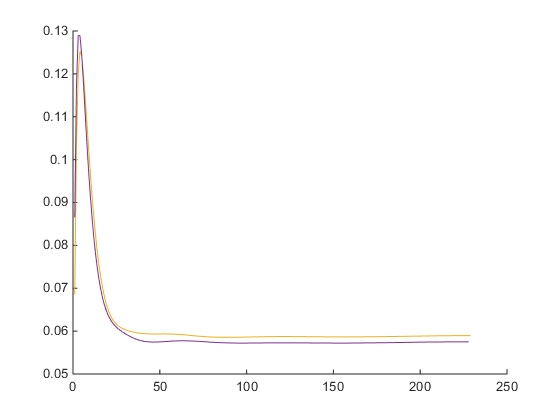
\includegraphics[width=10cm]{TESTimg.png}
 \caption{Test figure for list of figures.}
\label{Cd_mesh_ind}
\end{figure}
 %





\newpage
\bibliographystyle{unsrt}
\nocite{*}

\bibliography{ref}

\end{document}

% \begin{equation}
% C_{d,\,induced} = \frac{C_{l}^{2}}{\pi\, AR\, e}
% \label{DragEq}
% \end{equation}

% \begin{table}[H]
% \caption{Spatial discretization schemes and the pressure-velocity coupling for the 2D airfoil case.}
% \vspace{0.2cm}
% \centering
% \begin{tabular}{ll}
% Pressure-Velocity Coupling & Coupled \\
% Spatial Discretization $\rightarrow$ \textbf{Gradient} & Least Square Cell Based \\
% Spatial Discretization $\rightarrow$ \textbf{Pressure} & Second Order \\
% Spatial Discretization $\rightarrow$ \textbf{Density} & Third Order MUSCL \\
% Spatial Discretization $\rightarrow$ \textbf{Momentum} & Second Order Upwind \\
% Spatial Discretization $\rightarrow$ \textbf{Intermittency} & Second Order Upwind \\
% Spatial Discretization $\rightarrow$ \textbf{Turbulent Kinetic Energy} & Third Order MUSCL \\
% Spatial Discretization $\rightarrow$ \textbf{Specific Dissipation Rate} & Third Order MUSCL \\
% Spatial Discretization $\rightarrow$ \textbf{Energy} & Second Order Upwind \\
% Pseudo Transient & On \\
% High Order Term Relaxation & On \\
%  & Second Order Implicit
% \end{tabular}
% \label{solvmeth}
% \end{table}

% \begin{table}[H]
% \centering
% \caption{Solution controls used for in the Ansys solver for the 2D airfoil.}
% \begin{tabular}{lr}
% Pressure & 0.3 \\
% Momentum & 0.2 \\
% Turbulent Kinetic Energy & 0.6 \\
% Specific Dissipation Rate & 0.5 \\
% Energy & 0.9 \\
% \end{tabular}
% \label{solcont}
% \end{table}

% \begin{equation}
% \label{bl_flat_plate}
% \delta_{max} = max(0.382xRe_{x}^{-1/5})
% \end{equation}

% \begin{table}[H]
% \centering
% \caption{The settings and quality of the coarse and fine mesh.}
% \begin{tabular}{lccc}
% \multicolumn{1}{c}{\textbf{Mesh settings}} && \textbf{Coarse} & \textbf{Fine}\\
% Number of inflation layers && 51 & 51\\
% Growth rate of inflation layers && 1.1 & 1.1\\
% First layer thickness &$[m]$ & 6e-6  & 5e-6 \\
% Number of divisions && 1101 & 1351\\
% Body of influence element size &$[m]$ & 6e-2 & 6e-2 \\
% Bulk max size/max face size &$[m]$ & 0.20/0.20  & 0.10/0.10 \\
% Bulk growth rate &&1.050 & 1.050\\
% Total number of nodes && 180000 & 245000\\
% \multicolumn{1}{c}{\textbf{Mesh quality}} && \textbf{Coarse} & \textbf{Fine}\\
% Max aspect ratio && 179.13 & 193.81\\
% Average aspect ratio && 15.694 & 15.418\\
% Max skewness && 0.72632 & 0.7631\\
% Average skewness && 0.13813& 0.12419\\
% \end{tabular}
% \label{meshsettings}
% \end{table}

% \begin{table}[H]
% \caption[Mesh independence 2D.]{The results of the two different meshes combined with the relative difference between them.}
% \centering
% \begin{tabular}{lccr}
%  & \textbf{Coarse}& \textbf{Fine} & \textbf{Relative difference} \\
% Mesh nodes & 180 000 & 245 000 & 36.1\% \\
%  $C_D$ & 0.00790 & 0.00740 & 6.73\% \\
% $C_L$ & 0.368 & 0.366& 0.450\% \\
% $\frac{L}{D}$ & 46.3 & 49.42 & 6.74\% \\
% \end{tabular}
% \label{meshilainen}
% \end{table}

% \begin{table}[H]
% \centering
% \caption{Lengths and diameters in the computational domain for the 3D wing case I.}
% \begin{tabular}{lcc}
% Domain Forward/Backward 	&$[m]$ 		& 6.0/20 \\
% Domain Left/Right 			&$[m]$ 		& 8.0/8.0 \\
% Domain Up/Down 				&$[m]$ 		& 5.0/5.0 \\
% \end{tabular}
% \label{domainsizeetc3d1}
% \end{table}

% \begin{table}[H]
% \centering
% \caption[Computational domain and bluff body geometry, 3D wing case I.]{Measurements in the computational domain for the 3D wing case I along with the bluff body measurements. The origin is located in the wing root at leading edge, forward is positive x-axis and left is as wing extends.}
% \begin{tabular}{lcc}
% Bluff Body Forward/Backward 	&$[m]$ 		& 1.0/3.0 \\
% Bluff Body Straight Up/Down		&$[m]$ 		& 1.4/1.6 \\
% Bluff Body Radius From Front	&$[m]$ 		& 0.3 \\
% Bluff Body Radius Along Sides	&$[m]$ 		& 0.2 \\
% BoI I Forward/Backward 			&$[m]$ 		& 2.0/4.0 \\
% BoI I Left/Right 			 	&$[m]$ 		& 4.2/2.0 \\
% BoI I Body Up/Down 			 	&$[m]$ 		& 1.4/1.4 \\
% BoI II Backward From BoI I 		&$[m]$ 		& 16 \\
% BoI II Left/Right 			 	&$[m]$ 		& 4.2/2.0 \\
% BoI II Body Up/Down 		 	&$[m]$ 		& 0.8/0.8 \\
% \end{tabular}
% \label{domainsizeetc3d2}
% \end{table}

% \begin{table}[H]
% \centering
% \caption{The settings and quality of the mesh.}
% \begin{tabular}{lcc}
% \multicolumn{3}{c}{\textbf{Mesh settings}}  \\
% Bulk max size/max face size &$[m]$ & 0.80/0.80  \\
% Min size &$[m]$ & 0.10  \\
% Bulk growth rate && 1.30 \\
% Total number of nodes && 222000 \\
% \multicolumn{3}{c}{\textbf{Mesh quality}} \\
% Max skewness && 0.799 \\
% Average skewness && 0.220
% \end{tabular}
% \label{meshsettings13d}
% \end{table}

% \begin{table}[H]
% \centering
% \caption{Body sizing for the BoI's and edge sizing along the leading edge.}
% \begin{tabular}{lcc}
% \multicolumn{3}{c}{\textbf{Mesh quality}} \\
% BoI I element size 		&$[m]$ & 0.13 \\
% BoI II element size 	&$[m]$ & 0.20 \\
% BoI I min size 			&$[m]$ & 0.08 \\
% BoI II min size 		&$[m]$ & 0.08 \\
% Edge sizing along leading edge &$[m]$& 0.10 \\
% \end{tabular}
% \label{boiboiboi3d}
% \end{table}

% %Use Bibtex for references and the \texttt{cite} command to refer to the sources. See the .bbl file. Note - there are more available entries than you find in the file. Add your references as appropriate entries and compile at least three times. Citation: The first is to a web page~\cite{website:Tornado}. The second to a journal paper (article)~\cite{laurence:boundary}, and the third to a book~\cite{blazek:cfd}.

% %\begin{equation}
% %\alpha = \sqrt{\alpha^{2}}
% %\label{root}
% %\end{equation}
% %\pagebreak
% %\chapter{Bibliography}


% \pagebreak
% \appendix
% \chapter{Matlab Code for NACA 4-digit series airfoil}
% \lstset{columns=fullflexible, basicstyle=\ttfamily}
% Please note that if the resolution $n$ is set too high there might be problems when importing the coordinate file into Workbench Geometry.
% \begin{lstlisting}
% % function[M1,M2] = NACA4digit(NACA,c,n,cut) %Comment NACA,c,n and cut in
% % code if function calling is to be used

% clear all
% close all
% clc


% \end{lstlisting}
